\documentclass[12pt, a4paper]{report}

\usepackage{url}
\usepackage[utf8]{inputenc}
\usepackage{graphicx}
\usepackage{hyperref}
\usepackage{textcomp}

\usepackage[
    backend=biber,
    style=alphabetic,
    sorting=ynt
]{biblatex}
\addbibresource{darwinsquest.bib}

\graphicspath{{img/}} % configuring the graphicx package globally

\title{
    \begin{figure}[ht]
    \centering{}
    
\includegraphics[width=\textwidth]{logo} % remember best practice without extension, NO img/logo, img/logo.png or logo.png, but logo is enough
    \end{figure}
}
\author{
    Enrico Marchionni\\
    \texttt{enrico.marchionni@studio.unibo.it}
    \and
    Francesco Cipollone\\
    \texttt{francesco.cipollone@studio.unibo.it}
    \and
    Raffaele Marrazzo\\
    \texttt{raffaele.marrazzo@studio.unibo.it}
}
\date{\today}

\begin{document}

\maketitle

\begin{abstract}

    DarwinsQuest \cite{ontheoriginofspiecies} is a multi-level structured videogame set in a post apocalyptic world,
    shaken by climate change. The goal is to survive natural selection by completing numerous battles,
    after choosing your genetically modified banions\footnote{\emph{Banion} is the name we chose as game entities} (basic companions).

\end{abstract}

\tableofcontents

\chapter{Analysis}

\section{Requirements}

\subsubsection{Functional}

\begin{itemize}
    \item The game will open with a title screen, containing buttons to start/quit the game, \textit{and optionally a load button}.
    \item \textit{The player can choose between three game modes: Normal, Hard, and Impossible.}
    \item At the beginning of the game, the player must be able to select a starter fight companion from a number of multiple choices.
    \item The game interface will consist of a side-scrolling 2D view, containing the player and enemies. Encountering one enemy will prompt a battle.
    \item \textit{The game has to manage an economic system that manages win and loss currency transactions.}
    \item The player's movement will be managed by tiles. Each tile can be a move, battle, or special tile.
        The movement will be determined by the use of a random value. Said value corresponds to the number of tiles that the player can move.
    \item The companions are able to evolve based on an evolution tree. Starting from a node, the player can only select one of its children's nodes.
        Once the player has unlocked one of the leaf nodes, the last tree node, the evolution in the said tree is completed.
        \textit{Multiple trees can be present at once, meaning that multiple evolution branches could be developed at once.}
    \item The player has to sequentially complete a series of levels, with increasing difficulty until meeting the final boss.
        The battles are engaged in 1v1 a turn-based combat fashion, with the ability to switch between companions or perform moves.
        Later in the game, 2v2 battles can be triggered. After winning a battle the player can choose an upgrade from the evolution tree.
    \item The player can save their progress during the game. The player can save their progress only in the board.
        It will not be possible to save during fights.
\end{itemize}

\subsubsection{Non Functional}

\begin{itemize}
    \item The battle needs to be challenging for the player and will require a careful strategic plan planning ahead. \label{challengingbattle}
    \item The game performances must be acceptable.
    \item The game has to be portable and compatible with Windows, MacOS, and Linux systems.
\end{itemize}

\section{Domain Model}

    The player can move inside the board map bounds. The map contains the player, the enemies, and special tiles such as the shop, bonus, and penalty tiles.
    There are some different kind of tiles:
\begin{itemize}
    \item \textbf{Move tile}: a generic tile that does not contain any battle or special characteristics;
    \item \textbf{Battle tile}: landing on this tile will prompt the beginning of a battle (battle tiles cannot be skipped, regardless of the drawn value).
        Losing said battle will make the player stuck on this tile, preventing them from proceeding further in the game until they beat the opponent;
    \item \textbf{Special tile}:
    \begin{itemize}
        \item \textbf{Bonus tiles}:
        \begin{itemize}
            \item Money gain;
            \item Casual companion stats increase;
        \end{itemize}
    \end{itemize}
    \begin{itemize}
        \item \textbf{Penalty tiles}:
        \begin{itemize}
            \item Money loss;
            \item Casual companion stats decrease;
        \end{itemize}
    \end{itemize}
\end{itemize}

    The player can own one or more fight companions. Each companion has an intrinsic elemental type, such as fire, water, grass, rock, air, electro,
    and is associated has a set of moves, which are divided into groups based on the companions' elemental type. A certain companion with a certain
    type only retains moves of its same elemental type plus neutral moves, e.g. A fire companion can only use fire moves and neutral moves,
    and cannot perform other types' moves.

    Banions in our game are the following:

\begin{table}[ht]
    \begin{center}
    \begin{tabular}{| c | c | c | c | c | c | c |}
        \hline
        Banion & Element \\ [0.5ex] % Fire & Water & Grass & Rock & Air & Electro
        \hline\hline
        fat bird & Air \\
        \hline
        blue bird & Air \\
        \hline
        bee & Air \\
        \hline
        bat & Electro \\
        \hline
        bunny & Electro \\
        \hline
        chameleon & Electro \\
        \hline
        angry pig & Fire \\
        \hline
        chicken & Fire \\
        \hline
        mushroom & Fire \\
        \hline
        trunk & Grass \\
        \hline
        radish & Grass \\
        \hline
        plant & Grass \\
        \hline
        rocks & Rock \\
        \hline
        turtle & Rock \\
        \hline
        rino & Rock \\
        \hline
        slime & Water \\
        \hline
        snail & Water \\
        \hline
        duck & Water \\
        \hline
    \end{tabular}
    \caption{\label{table:banions} Banions}
    \end{center}
\end{table}

    Elemental reactions, that are bounded to moves, are defined as follows:

\begin{table}[ht]
    \begin{center}
    \begin{tabular}{| c || c | c | c | c | c | c |}
        \hline
        Player \textbackslash Enemy & Air & Electro & Fire & Grass & Rock & Water \\ [0.5ex]
        \hline\hline
        Air         & - & * & * & - & + & + \\
        \hline
        Electro     & * & + & * & - & * & * \\
        \hline
        Fire        & * & * & * & + & * & - \\
        \hline
        Grass       & + & + & - & * & - & * \\
        \hline
        Rock        & - & * & * & + & * & * \\
        \hline
        Water       & - & * & + & * & * & * \\
        \hline
    \end{tabular}
    \caption{\label{table:elements} Elements}
    \end{center}
\end{table}

    \textit{Each companion in the game will have a personal set of statistics, such as attack (ATK), defense (DEF), health points (HP).
    The values make up the base statistics of a certain companion.}

    In every level, there are two player entities: the player and the opponent (NPC). These entities deploy their companions, which will fight 1v1.
    A level consists of a selection phase, a battle phase, and leveling phase:
\begin{itemize}
    \item \textbf{Selection phase}: before battling the player has to choose the first companion in his battle lineup from his current team;
    \item \textbf{Battle phase}: during the player's fight turn, it is possible to switch their active companion to a different one (the team must have more than a single companion), 
        or the player can perform a move. Upon the player's active companion's defeat, they will be forced to switch to another one. 
        If the player is out of eligible companions the fight is over. In 2v2 battles, the player will deploy two of their companions. 
        It will be possible to select which of the two enemy companions to attack while respecting each other turns.
    \item \textbf{Leveling phase}: upon the player's victory, you will be prompted to choose an upgrade from the evolution tree, starting from any of the lastly unlocked nodes.
\end{itemize}

    The fight mechanics are considered a project challenge for their complexity \ref{challengingbattle}, from the elemental reaction logic to the moves management.

    The game currency can be obtained by winning battles and from bonus tiles (see ahead).
    Losing a battle or landing on a Money loss tile will decrease the player's money amount.
    Money can be used to purchase items, such as potions to temporarily increase your companion statistics, and companions from the in-game shop.

    Modelling an evolution tree is considered a challenge because it requires designing a complex branching system that accurately reflects the evolution of the companions in the game. 
    The tree must be visually appealing and easy to navigate, while also ensuring that each node is balanced and offers meaningful choices to the player. 
    The designer must also consider how to balance the evolution of multiple trees simultaneously and ensure that the player does not become overwhelmed with too many choices. 
    Additionally, the evolution tree must be designed to fit seamlessly into the game's mechanics and narrative.

\chapter{Design}

\section{Architecture}

    This projects is developed in \href{https://en.wikipedia.org/wiki/Model%E2%80%93view%E2%80%93controller}{MVC} (Model, View and Controller) architecture.
    In out architecture the \textbf{Controller} is the entry point of the application. It instantiates the \textbf{View} that instantiate, in turn, the
    \textbf{Controller} main class for interaction between \textbf{View} and \textbf{Controller}. The \textbf{Model} is instantiated by the \textbf{Controller}
    at the right moment, following MVC pattern.

    In our architecture the main classes are \textbf{JavaFXApplication} (View), \textbf{ControllerImpl} (Controller) and \textbf{EngineImpl} (Model). The
    first one is responsible for the collection of input and shows the output, the third one is the logic of the game and the second one is the link between them.

    % \begin{figure}[h]
    % \centering{}
    % 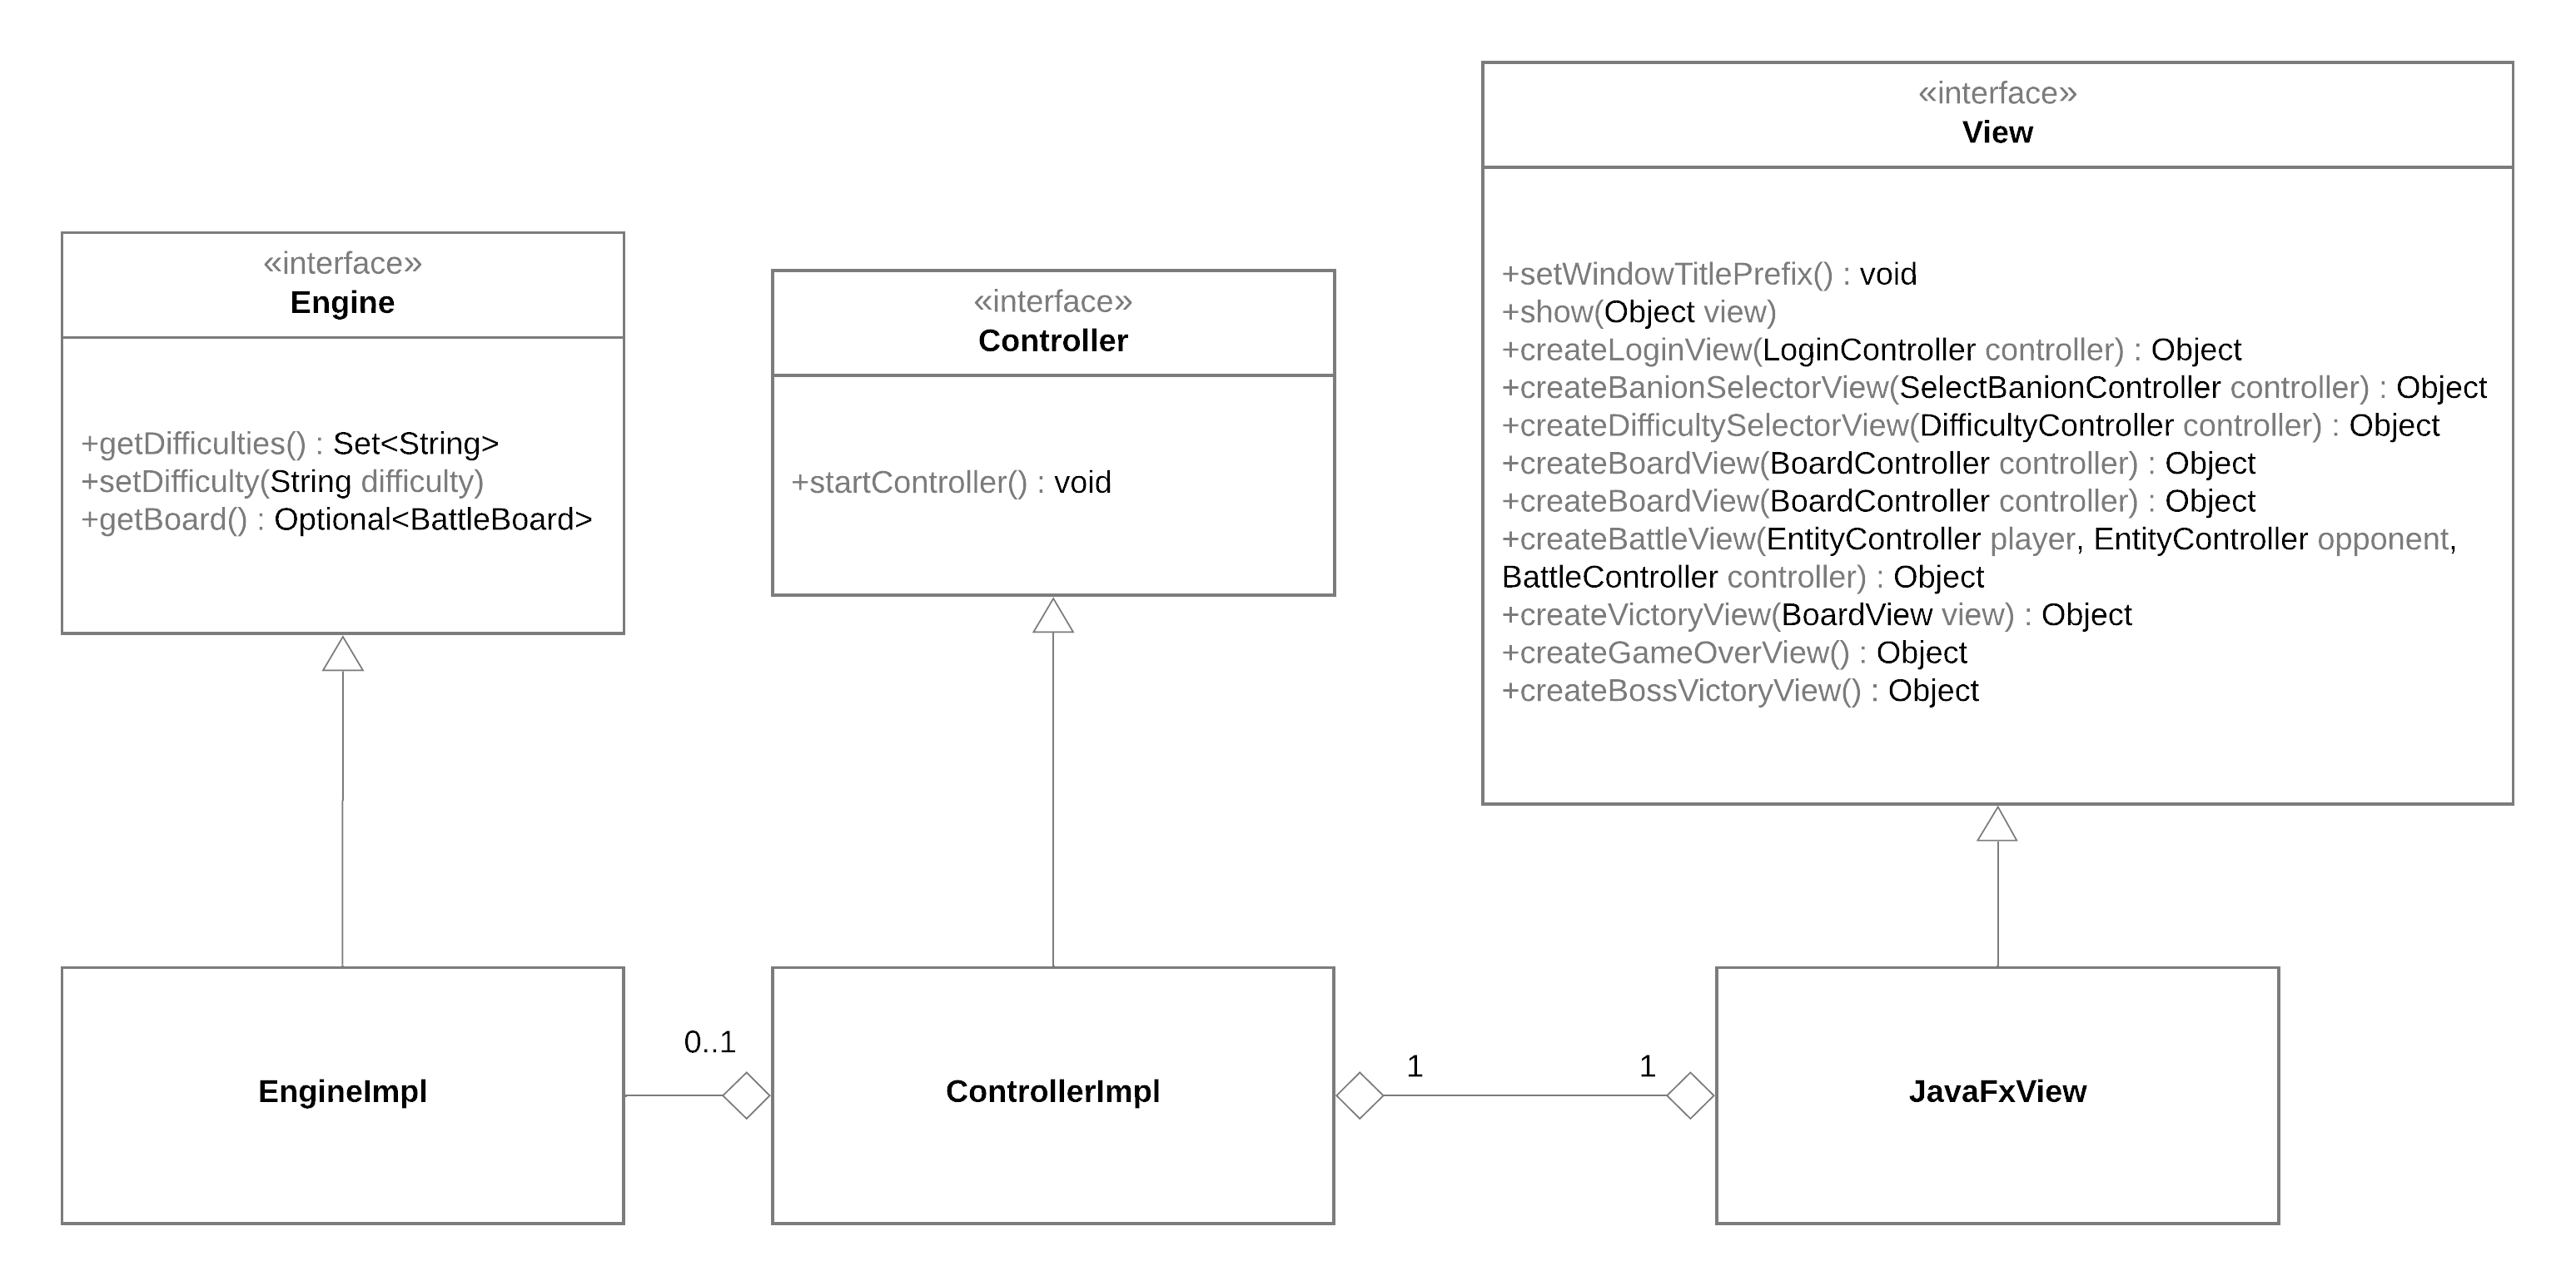
\includegraphics[width=\textwidth]{mvc}
    % \end{figure}

\section{Details}

    \dots

    \subsection*{Enrico Marchionni}

        \subsubsection{Game Difficulty}

            \paragraph{Problem}
            
            Giving the possibility to choose between different thought games.
            Each difficulty should determine for example the number of tiles for the \emph{Board}, the moving \emph{Strategy} in it,
            the number and \emph{Element} of the \emph{Opponent}'s \emph{Banion}s, the \emph{AI} for each \emph{Opponent}...
            A requirement is that this problem has to be resolved in an extendible way.
            So once the system is built, adding a difficulty must be easy and fast according to \emph{OCP} (open closed principle).

            \paragraph{Solution}

            The element \emph{Board} is the main entity of this game because it determines how much
            levels have to be completed to win the game. So the main \emph{Model} class that is responsible for
            the difficulties is the \emph{Engine} class. It retrieves the \emph{Board} and everything else go by itself
            only by selecting the \emph{Difficulty}. The difficulty has the goal to decide the \emph{Board} \emph{Strategy} of
            movement, the number of levels and the \emph{AI} associated with the \emph{Opponent}. Each \emph{Opponent} will
            be created by the \emph{Board} at the right moment through an \emph{OpponentFactory} that was created by the \emph{Difficulty}
            itself.

            \begin{figure}[ht]
            \centering{}
            \caption{UML difficulty}
            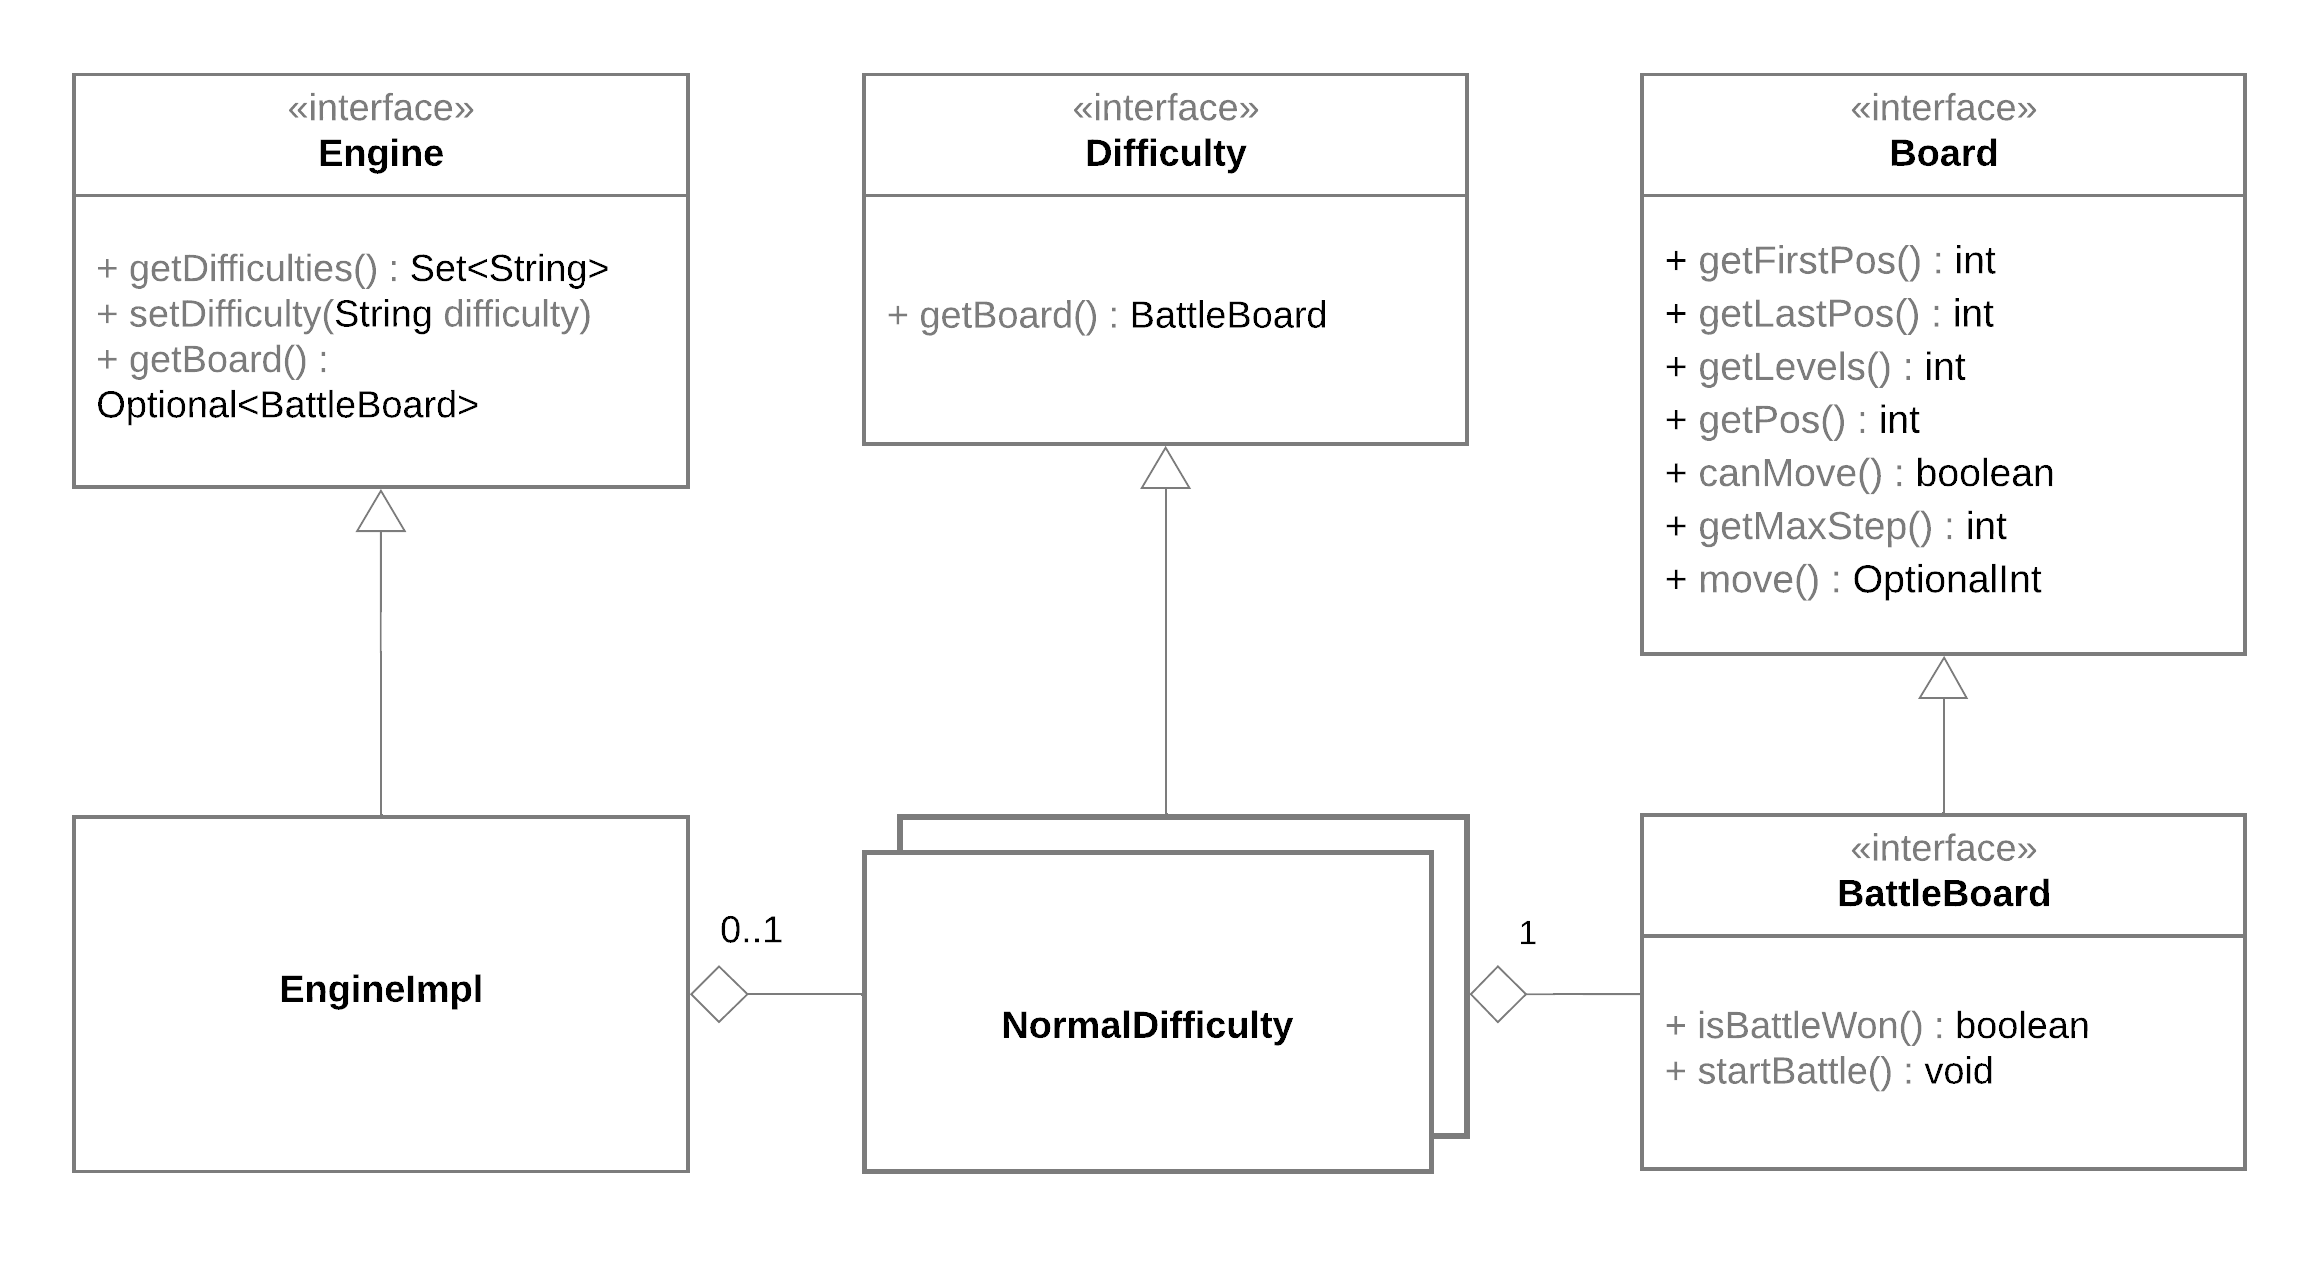
\includegraphics[width=\textwidth]{difficulty}
            % \label{img:difficulty}
            % \ref{img:difficulty}
            \end{figure}

            \paragraph{Pattern}

            The \emph{Difficulty} decides the \emph{Board} step of movement by passing a \emph{PositiveIntSupplier} to \emph{Board} constructor via \emph{Strategy}.
            Furthermore the \emph{Difficulty} decides also the \emph{OpponentFactory} implementation to pass to the \emph{Board} via \emph{Strategy}.
            The \emph{OpponentFactory} can be considered ad Abstract Factory because every single implementation of \emph{Difficulty} could pass
            a different implementation of \emph{OpponentFactory} to the relative \emph{BattleBoard}.
            
        \pagebreak

        \subsubsection{\emph{Element}s, \emph{Move}s and \emph{Banion}s Generation}

            \paragraph{Problem}
            
            Generating game entities: \emph{Element}, \emph{Move} and \emph{Banion}. Our game needs a consistent number of \emph{Banion}s \ref{table:banions} to be playable.
            It would better if they could be the same every time the application starts: same names, same sprites, same moves...
            Independently from the user progresses it would be nice for a user to choose between the same set of Banions at the beginning of every new the game.

            \paragraph{Solution}

            The problem is that somehow these entities has to be created, so how I decided to do that is the solution.
            At the beginning I started from the generation of \emph{Element}s \ref{table:elements} by coding each one in Java classes.
            The two main problems I observed were the expansion of classes and the inability to easily and quickly add new ones.
            After that I took time to think at a more extendible and cleaner solution, at the end I decided to go for the deserialization.
            I decided to create in the MVC \emph{Controller} a system to deserialize entities from file.
            In specific I chose \textit{.json}, using \href{https://github.com/google/gson}{Gson} library.
            
            I also wanted to make sure to avoid duplication of information.
            We decided that every single entity must be identifiable by name.
            So I created three files, one for each entity to generate, following this structure:
            \begin{itemize}
                \item \emph{Element} \textrightarrow independent from the other entities;
                \item \emph{Move} \textrightarrow dependent from \emph{Element} entities (each \emph{Move} is associated with one \emph{Element});
                \item \emph{Banion} \textrightarrow dependent from \emph{Element} and \emph{Move} entities (each \emph{Banion} is associated with one \emph{Element} and 4 \emph{Move}s);
            \end{itemize}

            I also decoupled file reading from entities generation.
            I put in the \textit{darwinsquest.config} package classes to read from file while in \textit{darwinsquest.config} I put the Factories according to \emph{SRP} (single responsibility principle).

            \paragraph{Pattern}

            The entities are created by using \emph{Factory} pattern.
            \emph{ElementFactory}, \emph{MoveFactory} and \emph{BanionFactory} retrieves the deserialized data with the shape of a set.

            \paragraph{Comments}

            Following this scheme in future it could be easily add the functionality of writing a system to save user progress.
            This would consist essentially on storing user \emph{Banion}s data in a folder (ex. \emph{.darwinsquest} in the user folder) and reload them after the login operation.
            For what concerns \emph{User} and \emph{Board} progresses serialization it should be thought in organization, and it would be integrated with the serialization/deserialization of entities.

        \pagebreak

        \subsubsection{\emph{Sprite}s}

            \paragraph{Problem}

            Each \emph{Banion} should be represented by a \emph{Sprite} in the \emph{View}.

            \paragraph{Solution}

            I considered that each \emph{Banion} is uniquely identified by its name.
            So I decided to put the necessary data in the same \textit{.json} file that contained also the \emph{Banion}s information.
            By doing that I created a \emph{BanionsSpriteFactory} class in the \emph{View} that has to read \emph{Sprite} record (it contains \emph{Banion} .png information).
            Each banion will be associated in the \emph{View} to its \emph{Sprite} by its name (this can be seen in \emph{ChooseBanionMenuView} constructor).

            \paragraph{Pattern}

            \emph{BanionsSpriteFactory} is a \emph{Factory} of \emph{Banion}'s \emph{Sprite}s.
            
        \pagebreak

        \subsubsection{View}

            \paragraph{Problem}

            How to separate concerns in the chosen \emph{JavaFX} library.
            How to decouple style from showing controls, for example how to specify each \emph{Scene} font in a \emph{DRY} (don't repeat yourself) way.

            \paragraph{Solution}

            I started by using \textit{.css} files to specify style and \textit{.fxml} to specify layouts for each Container.
            I created a Controller for each Container.

            \paragraph{Pattern}

            
        \pagebreak

    \subsection*{Francesco Cipollone}

    \dots

    \subsection*{Raffaele Marrazzo}

    \dots

\chapter{Deployment}

    \dots

\section{Automatized testing}

    \dots

    \subsection*{Enrico Marchionni}

    \dots

    \subsection*{Francesco Cipollone}

    \dots

    \subsection*{Raffaele Marrazzo}

    \dots

\section{Work strategy}

    \dots

\section{Development notes}

    \dots

    \subsection*{Enrico Marchionni}

    \dots

    \subsection*{Francesco Cipollone}

    \dots

    \subsection*{Raffaele Marrazzo}

    \dots

\subsection{Example}

    \dots

\chapter{Final comments}

    \dots

\section{Self-evaluation and future improvements}

    \dots

    \subsection*{Enrico Marchionni}

    \dots

    \subsection*{Francesco Cipollone}

    \dots

    \subsection*{Raffaele Marrazzo}

    \dots

\section{Difficulties and comments to teachers}

    \dots

    \subsection*{Enrico Marchionni}

    \dots

    \subsection*{Francesco Cipollone}

    \dots

    \subsection*{Raffaele Marrazzo}

    \dots

\appendix

\chapter{User guide}

    \dots

\chapter{Laboratory}

\section{enrico.marchionni@studio.unibo.it}

\begin{itemize}
    \item Lab 04: \url{https://virtuale.unibo.it/mod/forum/discuss.php?d=113869#p169173}
    \item Lab 05: \url{https://virtuale.unibo.it/mod/forum/discuss.php?d=114647#p169723}
    \item Lab 06: \url{https://virtuale.unibo.it/mod/forum/discuss.php?d=115548#p171159}
    \item Lab 07: \url{https://virtuale.unibo.it/mod/forum/discuss.php?d=117044#p173058}
    \item Lab 08: \url{https://virtuale.unibo.it/mod/forum/discuss.php?d=117852#p174127}
    \item Lab 09: \url{https://virtuale.unibo.it/mod/forum/discuss.php?d=118995#p175326}
    \item Lab 10: \url{https://virtuale.unibo.it/mod/forum/discuss.php?d=119938#p176522}
    \item Lab 11: \url{https://virtuale.unibo.it/mod/forum/discuss.php?d=121130#p177368}
    \item Lab 12: \url{https://virtuale.unibo.it/mod/forum/discuss.php?d=121885#p178425}
\end{itemize}

\printbibliography

\end{document}